\documentclass{article}
\usepackage[T1]{fontenc}
\usepackage{lmodern}
\usepackage{graphicx}
\usepackage{amsmath,amssymb}
\usepackage[a4paper,margin=2cm]{geometry}
\usepackage[absolute,overlay]{textpos}
\setlength{\TPHorizModule}{1mm}
\setlength{\TPVertModule}{1mm}
\usepackage[indonesian]{babel}
\usepackage{hyperref}
\setlength{\emergencystretch}{2em}
% unit: Halaman 24

\begin{document}

% === Halaman 24 (llm) ===

\vspace{173.45mm}

\textcolor{red}{\textbf{Penggunaan OTP pada perang dingin antara AS dan Uni Soviet}}

\vspace{238.79mm}

\textcolor{red}{\textbf{The Moscow--Washington hotline [1963]:}}
\begin{itemize}
    \item Komunikasi antara AS dan Uni Soviet menggunakan hotline komunikasi langsung antara pemimpin AS dan Uni Soviet.
    \item Hotline difasilitasi dengan peralatan OTP yang bernama ITT Intelex Teletype L015
\end{itemize}

\begin{itemize}
    \item ITT Intelex Teletype dikembangkan setelah krisis rudal Cuba untuk menghindari perang nuklir
\end{itemize}

\vspace{10mm}

\begin{itemize}
    \item \textcolor{red}{\textbf{ITT Intelex Teletype mengenkripsi pesan menggunakan OTP}}
    \begin{itemize}
        \item Kunci \textit{one-time pad} disimpan di dalam pita magnetic yang diterbangkan antara Washington DC dan Moscow.
    \end{itemize}
\end{itemize}

\vspace{10mm}

Sumber: John H Reif, History of Computing, Duke University

% deskripsi: Foto mesin ITT Intelex Teletype L015 yang digunakan untuk hotline Moskow-Washington.
% bbox normalisasi: [0.6970, 0.0000, 0.9260, 0.5840]
\begin{textblock*}{48.09mm}(146.37mm,0.00mm)
\noindent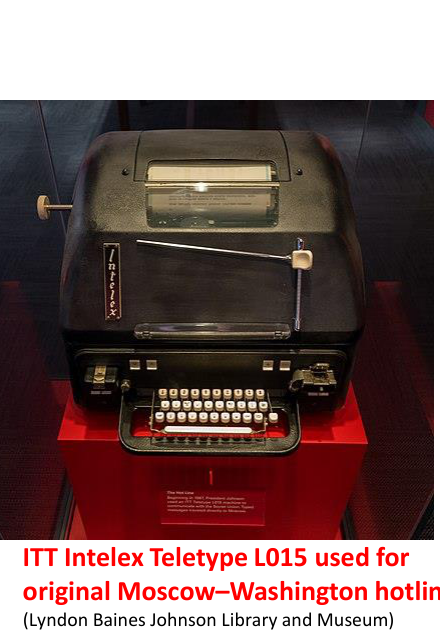
\includegraphics[width=48.09mm,height=173.45mm]{../../images/llm/page_024_img_01.png}%
\end{textblock*}

% deskripsi: Foto udara gedung Pentagon di Arlington County, Virginia, AS.
% bbox normalisasi: [0.5020, 0.6410, 0.6680, 0.8950]
\begin{textblock*}{34.86mm}(105.42mm,190.38mm)
\noindent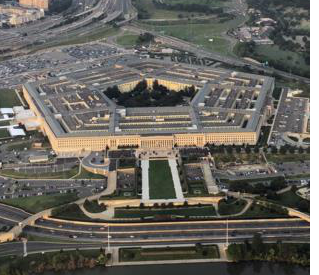
\includegraphics[width=34.86mm,height=75.44mm]{../../images/llm/page_024_img_02.png}%
\end{textblock*}

% deskripsi: Foto gedung Kremlin di Moskow, Rusia.
% bbox normalisasi: [0.7730, 0.6410, 0.9710, 0.8950]
\begin{textblock*}{41.58mm}(162.33mm,190.38mm)
\noindent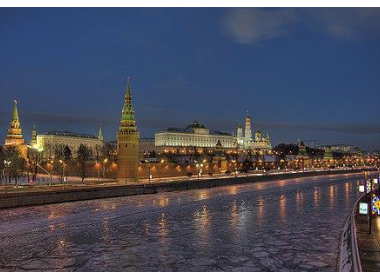
\includegraphics[width=41.58mm,height=75.44mm]{../../images/llm/page_024_img_03.png}%
\end{textblock*}

% deskripsi: Panah merah dua arah yang menunjukkan komunikasi antara Pentagon dan Kremlin.
% bbox normalisasi: [0.0600, 0.1080, 0.9400, 0.9120]
\begin{textblock*}{184.80mm}(12.60mm,32.08mm)
\noindent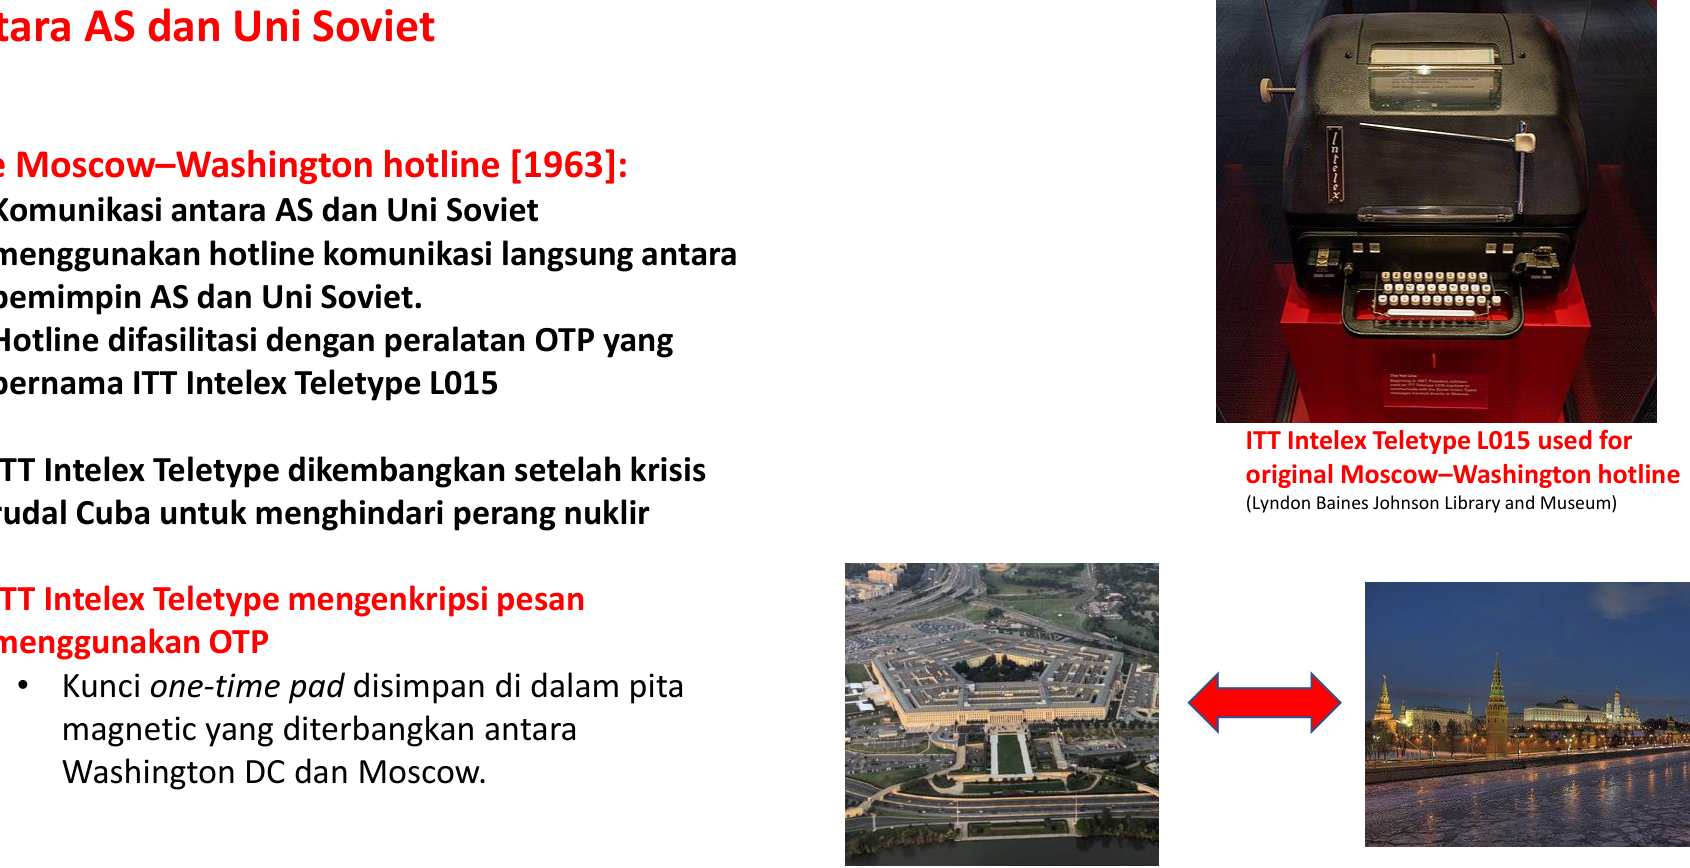
\includegraphics[width=184.80mm,height=238.79mm]{../../images/llm/page_024_img_04.png}%
\end{textblock*}

% bbox perkiraan otomatis: Panah merah dua arah yang menunjukkan komunikasi antara Pentagon dan Kremlin.

\end{document}
